% CPAIOR 2027 -- draft 2 (2026-10-04), rewritten after CPAIOR 2020/2026 papers
% (structure, formal problem definition, algorithm box, protocol, tone).
% Needs llncs.cls and splncs04.bst from the template, references.bib and
% fig_effort.pdf (python ML/paper/fig_effort.py) in the same folder.
% Every number comes from ML/results (see ML/STATUS.html); the script that
% produced each table is named in a comment above it.
\documentclass[runningheads]{llncs}
%
\usepackage[T1]{fontenc}
\usepackage{newtxtext}
\usepackage[varvw]{newtxmath}
\usepackage{graphicx}
\usepackage{booktabs}
\usepackage{algorithm}
\usepackage{algpseudocode}
%
\begin{document}
%
% working title: OR x ML for electric truck driver scheduling
\title{Learning Charging and Rest Decisions for Electric Trucks from a
Stochastic Look-Ahead Policy}
\titlerunning{Learning Charging and Rest Decisions from a Look-Ahead Policy}
%
\author{C\'eline Pagnier\inst{1}\orcidID{0009-0009-7276-9525} \and
Steffen J. S. Bakker\inst{2,3}\orcidID{0000-0002-2656-3827}}
%
\authorrunning{C. Pagnier and S. J. S. Bakker}
% TODO: affiliations 2 and 3 for the second author
\institute{Department of Industrial Economics and Technology Management, Norwegian University of Science and Technology, Trondheim, Norway}
%
\maketitle
%
\begin{abstract}
We consider the online scheduling of charging stops, breaks and daily rests
for a battery-electric truck under the EU driving-time regulation, with
uncertain travel times. A stochastic rolling-horizon look-ahead policy that
solves a mixed-integer program for every candidate action at every stop
reaches a median gap of 2.1\% to the hindsight optimum, but requires about a
minute of solver time per decision. We study to what extent a policy learned
by imitation of this look-ahead can replace it. The learned policy is trained
on the costs that the look-ahead computes for every candidate action and is
executed behind a symbolic shield that enforces the regulation. On 125
held-out routes, it is statistically indistinguishable from the look-ahead
($+0.17\pm0.30$\% route duration) and never violates the regulation, at 3\,ms
per decision. It generalizes to battery capacities, charger powers and
charger spacings within the training range, but not to chargers slower than
those seen in training, nor to routes on which charger power varies along the
route, where every policy trained on uniform routes loses at least 3.7
percentage points while the look-ahead loses nothing. On such routes, data
aggregation (DAgger) with the look-ahead as expert recovers about half of the
loss using 1{,}781 expert queries, which is as good as or better than adding
up to 8{,}246 decisions of whole-route demonstrations.
\keywords{Imitation learning \and Rolling-horizon look-ahead \and Electric
vehicles \and Hours-of-service regulation \and Data aggregation}
\end{abstract}
%
%
\section{Introduction}
\label{sec:intro}

The electrification of road freight requires heavy-duty trucks to recharge
during long-haul trips. For a battery-electric truck, charging cannot be
planned independently of the driver: EU Regulation 561/2006~\cite{eu561}
imposes breaks after 4.5 hours of driving and daily rests within each
working day, and these stops are natural opportunities to charge. The joint
problem of when to charge, for how long, and when to break or rest is further
complicated by uncertain travel times, which make a plan computed at departure
quickly obsolete. Decisions are therefore taken online, at each stop of the
route.

Electric vehicle routing with recharging~\cite{schneider2014,montoya2017} and
vehicle scheduling under drivers' working-hour
regulations~\cite{goel2009,goel_vidal2014} have been studied extensively, but
mostly separately and in deterministic settings. In a companion
paper~\cite{pagnier_bakker_journal}, we formulated the joint problem as a
mixed-integer program (MIP) and compared several online policies under
travel-time uncertainty. The best of them is a stochastic rolling-horizon
look-ahead (LA)~\cite{powell2022}, which evaluates every candidate action at
the current stop by solving the MIP over the next 24 hours for 25 sampled
travel-time scenarios. The LA reaches a median gap of 2.1\% to the hindsight
optimum. However, each decision takes about one minute of solver time, it
requires a commercial MIP solver, and the computation must be repeated for
every route, vehicle and charging network.

Learning a policy from an expensive optimization procedure is a recurring
idea in the integration of machine learning and combinatorial
optimization~\cite{bengio2021,amos2023}; learning to branch by imitation of
strong branching is a well-known example~\cite{khalil2016,gasse2019}. In this
paper, we apply this idea to the LA and ask two questions. First, can a policy
learned by imitation match the LA on the routes it was trained for, without
violating the regulation? Second, under which changes of the vehicle or the
charging network does the learned policy remain reliable, and how should
solver time be spent when it does not?

Our contributions are as follows. (i) We propose a cost-sensitive imitation
of the LA that uses the costs the LA computes for every candidate action,
combined with a symbolic shield that enforces the regulation independently of
the learned model. (ii) We show on 125 held-out routes that the learned policy
matches the LA with no rule violation, at 3\,ms per decision. (iii) We
characterize its generalization across battery capacities, charger powers and
charger spacings, and identify routes on which charger power varies as a case
where all learned policies fail. (iv) We show that, on these routes, data
aggregation~\cite{ross2011} with the LA as expert is a more efficient use of
solver time than additional demonstrations.

The rest of the paper is organized as follows. Section~\ref{sec:related}
reviews related work. Section~\ref{sec:problem} defines the problem, the LA
and the hindsight oracle. Section~\ref{sec:method} presents the learning
method, and Sect.~\ref{sec:exp} reports the computational experiments.
Section~\ref{sec:conclusion} concludes.

\section{Related Work}
\label{sec:related}

\subsubsection{Electric vehicles and driving-time regulations.}
The electric vehicle routing problem with time windows and recharging
stations was introduced by Schneider et al.~\cite{schneider2014}, and Montoya
et al.~\cite{montoya2017} showed the importance of modelling the nonlinear
charging function. Goel~\cite{goel2009} studied vehicle scheduling and routing
under the EU regulation on drivers' working hours, and Goel and
Vidal~\cite{goel_vidal2014} compared the regulations of several countries.
These works consider deterministic travel times and, to the best of our
knowledge, do not combine charging decisions with the full set of break and
rest rules. The companion paper~\cite{pagnier_bakker_journal} addresses this
combination under uncertainty with MIP-based policies.

\subsubsection{Learning from optimization experts.}
Machine learning has been used to replace or accelerate expensive components
of optimization algorithms~\cite{bengio2021}. Khalil et al.~\cite{khalil2016}
and Gasse et al.~\cite{gasse2019} learn branching rules by imitating strong
branching, and amortized optimization~\cite{amos2023} more generally learns
to predict the solutions of a family of optimization problems. In imitation
learning, a policy trained on the states visited by the expert can reach
states that the expert never visits; DAgger~\cite{ross2011} addresses this
covariate shift by querying the expert on the states visited by the learned
policy. In our setting, the expert is an optimization procedure that can be
queried at any state, which makes this approach directly applicable.

\subsubsection{Safety of learned policies.}
Shielding~\cite{alshiekh2018} restricts the actions of a learned policy to
those that a formal specification allows. We follow the same principle: the
legality of an action is never learned but checked against the regulation
before the learned model is consulted.

\section{Problem Definition}
\label{sec:problem}

\subsubsection{Route, uncertainty and state.}
A truck drives a fixed route of stops $i\in\{0,\dots,N\}$, from the origin
$0$ to the destination $N$. The set of stops is partitioned into charging
stations $K$, placed about every 60\,km as required on the core European
network~\cite{afir}, laybys $L$ where the driver can stop but not charge, and
customers $C$, each with a service time of 0.5\,h and possibly a time window
$[e_i,l_i]$. Leg $i$ goes from stop $i$ to stop $i+1$ and has a nominal travel
time $d_i$. Its realized travel time is $d_i\xi_i$, where
\begin{equation}
\xi_i=\min\{\xi^{\min}+\eta_i,\ \xi^{\max}\},\qquad
\eta_i\sim\mathrm{LogNormal}(\mu,\sigma^2),
\label{eq:xi}
\end{equation}
with $\xi^{\min}=8/9$ (an 80\,km/h nominal speed against the 90\,km/h speed
limiter), $\xi^{\max}=1.6$, and $(\mu,\sigma)$ calibrated so that
$\mathbb{E}[\xi_i]=1$ with a target coefficient of variation of 0.15. The
energy consumed on a leg follows a road-load model at the realized speed.
Both are revealed only once the leg has been driven. On arrival at stop $i$,
the state $s_i=(t_i,\epsilon_i,c_i)$ consists of the arrival time $t_i$, the
battery energy $\epsilon_i$, and a vector $c_i$ of regulatory counters: driving
time since the last break, driving and on-duty time in the current shift,
time elapsed since the end of the last daily rest, the progress of a split
break, and the remaining numbers of reduced rests and extended shifts.

\subsubsection{Actions and regulation.}
At stop $i$, an action $a=(y,b,r)$ specifies whether the truck charges
($y=1$, only if $i\in K$), and either a break $b\in\{b_{45},b_{15},b_{30}\}$ or
a daily rest $r\in\{r_{11},r_9\}$ (of 11 or 9 hours), or neither. Together with
$y$, this gives a set $\mathcal{A}$ of twelve action types. A charging action
is completed by a charging duration $\tau\ge 0$. Following~\cite{eu561} and
Directive 2002/15/EC~\cite{eu2002_15}, driving between two breaks is limited to
4.5\,h, where the 45-minute break $b_{45}$ may be split into $b_{15}$ followed
by $b_{30}$; driving within a shift is limited to 9\,h, or 10\,h at most twice
per week; and a daily rest of 11\,h, or 9\,h at most three times per week, must
start at most 13\,h, or 15\,h for a reduced rest, after the end of the
previous one. We denote by $\mathcal{A}(s_i)\subseteq\mathcal{A}$ the set of
actions that are legal in state $s_i$. A route on which a limit is exceeded is
counted as infeasible.

\subsubsection{Charging and objective.}
The battery has a capacity $\epsilon^{\max}=500$\,kWh and must stay above
$0.2\,\epsilon^{\max}$. A station $k\in K$ rated at $P_k$\,kW charges at rate
$P_k$ up to $0.8\,\epsilon^{\max}$ and at $\min\{P_k,0.4\,\epsilon^{\max}/\text{h}\}$
above it; it has a known expected queueing time $Q_k$ (10\,min on average)
and a setup time of 10\,min. A break or rest taken at a station overlaps with
charging. For a policy $\pi$, the cost of a route is
\begin{equation}
z(\pi)=t_N+\beta\sum_{i\in C}\mathbf{1}\{t_i\notin[e_i,l_i]\},
\label{eq:obj}
\end{equation}
the arrival time at the destination plus a penalty $\beta=0.5$\,h per missed
time window, and the goal is to minimize $\mathbb{E}[z(\pi)]$.

\subsubsection{Look-ahead policy and hindsight oracle.}
Let $\Omega_i$ be a set of 25 travel-time scenarios sampled from
(\ref{eq:xi}) for the legs within 24\,h of stop $i$, and let $z^H(s_i,a,\omega)$
be the optimal value of the MIP of~\cite{pagnier_bakker_journal} over these
legs, with the first action fixed to $a$ and travel times $\omega$. The LA
selects
\begin{equation}
a_i^{\mathrm{LA}}\in\arg\min_{a\in\mathcal{A}(s_i)}\ \bar c(s_i,a),\qquad
\bar c(s_i,a)=\frac{1}{|\Omega_i|}\sum_{\omega\in\Omega_i}z^H(s_i,a,\omega),
\label{eq:la}
\end{equation}
where infeasible scenarios are penalized, and prefers a charging action when
its value is within 5\,min of the minimum. The MIPs are solved with Gurobi
through Pyomo; with eight parallel workers on a laptop, a decision takes 71\,s
on average (110\,s at charging stations). The \emph{oracle} solves the MIP
over the whole route with the realized travel times, which gives a lower bound
$z^\ast$ on the cost of any policy. We report the gap $(z(\pi)-z^\ast)/z^\ast$.

\section{Learning Method}
\label{sec:method}

\subsubsection{Training data.}
To compute~(\ref{eq:la}), the LA evaluates $\bar c(s,a)$ for every action
$a\in\mathcal{A}(s)$. Instead of recording only the selected action, we record
all of these values. Let $\mathcal{A}^F(s)\subseteq\mathcal{A}(s)$ be the
actions that are feasible in all scenarios. For $a\in\mathcal{A}^F(s)$, the
regression target is the regret
\begin{equation}
\rho(s,a)=\bar c(s,a)-\min_{a'\in\mathcal{A}^F(s)}\bar c(s,a'),
\label{eq:regret}
\end{equation}
and the binary label $\mathbf{1}\{a\in\mathcal{A}^F(s)\}$ is the target of a
feasibility model. A state therefore yields between 4 and 10 labelled
actions. Each pair $(s,a)$ is described by 95 features, 77 for the state (the
slack to each regulatory limit, the energy margin to the next stations, the
next three stations and two customers, a summary of the 24-hour window of the
LA, and the remaining route) and 18 for the action (e.g., its duration and
the slack it leaves at the next time window).

\subsubsection{Models.}
We train three models: a cost model $\hat c(s,a)$ for the regret, a
feasibility model $\hat p(s,a)$, and a model of the charging duration. With
gradient-boosted trees (LightGBM~\cite{ke2017}), each model is a separate
booster and the cost model minimizes a Huber loss. Each decision is weighted
by $w(s)=m(s)/(m(s)+2\,\mathrm{se}(s))$, where $m(s)$ is the difference between
the two best values of $\bar c(s,\cdot)$ and $\mathrm{se}(s)$ its standard
error over the scenarios, so that decisions on which the LA is indifferent
receive little weight. With neural networks (PyTorch~\cite{paszke2019}), each
model is a separate multilayer perceptron, and the cost model minimizes
\begin{equation}
\mathcal{L}(\theta)=\sum_{s}w(s)\Big[\sum_{a\in\mathcal{A}^F(s)}
\ell_\delta\big(\hat c_\theta(s,a)-\rho(s,a)\big)
+\lambda\,\mathrm{CE}\big(\mathrm{sm}(-\rho(s,\cdot)/T),\,\mathrm{sm}(-\hat c_\theta(s,\cdot)/T)\big)\Big],
\label{eq:loss}
\end{equation}
where $\ell_\delta$ is the Huber loss, $\mathrm{sm}$ the softmax over
$\mathcal{A}^F(s)$, and CE the cross-entropy, with $\delta=1$\,h, $T=0.25$\,h
and $\lambda=1$. The second term penalizes errors in the order of the actions
of a state rather than in their values. Without it, the network predicted the
cost of daily rests more accurately than the trees but ranked them worse, and
took an unnecessary daily rest on several short routes.

\subsubsection{Decision rule and shield.}
The learned policy selects
\begin{equation}
\hat\pi(s)\in\arg\min\big\{\hat c(s,a):\ a\in\hat{\mathcal{A}}(s),\
\hat p(s,a)\ge 0.5\big\},
\label{eq:policy}
\end{equation}
where $\hat{\mathcal{A}}(s)\subseteq\mathcal{A}(s)$ is computed by a symbolic
shield. The legal set $\mathcal{A}(s)$ and the actions that the regulation
makes mandatory are derived from the simulator's rules and are never
learned. The shield further removes an action if one of the regulatory
counters would exceed its limit when the next leg is driven with the 0.99
quantile of $\xi$, or if the duration of the stop would exceed the time left
before the next daily rest. The predicted charging duration is clipped to the
interval between the charge needed to reach the next station in the worst
case and a full battery.

\subsubsection{Data aggregation with the look-ahead as expert.}
The training states are those visited by the LA. Algorithm~\ref{alg:dagger}
adds states visited by the learned policy itself. The learned policy drives
the training routes (line~5); every state it visits that differs from the
states reached by the LA on the same route, and in which at least two actions
are admissible, is stored (line~6), and the LA is queried at that state with
its usual configuration (line~7). The policy is then retrained on all the
data collected so far (line~9). As a sanity check, we queried the LA again
at 24 states that it had visited itself: it selected the same action in all
24 cases, and the differences between the two evaluations of $\bar c$ were
within the scenario standard errors.

\begin{algorithm}[t]
\caption{Data aggregation with the look-ahead as expert}
\label{alg:dagger}
\begin{algorithmic}[1]
\Require training routes $\mathcal{R}$, LA data $\mathcal{D}_0$, number of rounds $R$
\State train $\hat\pi_0$ on $\mathcal{D}_0$
\For{$k=1,\dots,R$}
  \State $\mathcal{D}_k\gets\emptyset$
  \For{each route $q\in\mathcal{R}$}
    \State drive $\hat\pi_{k-1}$ on $q$ with its realized travel times
    \State $S\gets$ visited states that differ from the LA's on $q$, with $|\hat{\mathcal{A}}(s)|\ge2$
    \State evaluate $\bar c(s,a)$ with the LA for all $s\in S$, $a\in\mathcal{A}(s)$; add them to $\mathcal{D}_k$
  \EndFor
  \State train $\hat\pi_k$ on $\mathcal{D}_0\cup\dots\cup\mathcal{D}_k$
\EndFor
\State \Return $\hat\pi_R$
\end{algorithmic}
\end{algorithm}

\section{Computational Experiments}
\label{sec:exp}

\subsection{Protocol}
\label{sec:protocol}

\subsubsection{Instances.}
Routes are 800--1{,}200, 1{,}500--2{,}500 or 3{,}000--4{,}000\,km long, which
gives 39--61, 72--120 and 144--185 stops, and serve 1--3, 4--6 or 7--15
customers with no, tight (0.5--1\,h half-width), medium (1--3\,h) or large
(3--6\,h) time windows. The resulting 36 families have 25 routes each, and
each route has one travel-time realization. Routes with seeds 1--19 are used
for training (639 routes solved by the LA, 56{,}104 decisions), seeds 20--21
for model selection and early stopping (66 routes), and seeds 22--25 for
testing (125 routes). Each configuration is trained with three random seeds,
selected on the validation routes, and evaluated once on the test routes.

\subsubsection{Methods.}
We compare the following policies:
\begin{enumerate}
\item \emph{Greedy}, the rule-based policy of~\cite{pagnier_bakker_journal};
\item \emph{LA}, the look-ahead policy~(\ref{eq:la}), which is also the expert;
\item \emph{Trees}, the learned policy~(\ref{eq:policy}) with LightGBM models
  (63 leaves, depth 6, at most 1{,}200 rounds with early stopping);
\item \emph{Network}, the learned policy~(\ref{eq:policy}) with neural models
  (cost model with layers of 256, 256 and 128 units, other models with two
  layers of 128 units, AdamW, early stopping on the validation decisions);
\item \emph{MLP}, a scikit-learn network trained by squared error on each
  action separately, without~(\ref{eq:loss}), as a simpler neural baseline.
\end{enumerate}
The learned policies run on a CPU and use the full shield. The LA runs were
made on a laptop with four cores and on a 32-core Linux server, with Gurobi
12.0.

\subsubsection{Metrics.}
We report the gap to the oracle and, for each learned policy, the relative
difference in route duration with the LA, paired by route and averaged over
the three training seeds; $\pm$ denotes one standard error over routes. We
also report the number of routes on which the regulation is violated and the
computing time per decision.

\subsection{Comparison with the Look-Ahead Policy}
\label{sec:base}

% numbers: ML/scratch/cmp_test.py g99sr (3 seeds each, route mean over seeds)
\begin{table}[t]
\caption{Results on the 125 test routes. Relative route duration with
respect to the LA, paired by route and averaged over three training seeds.
The LA has a median gap of 2.1\% to the oracle, Greedy 4.8\%.}
\label{tab:base}
\centering
\begin{tabular}{lrrrr}
\toprule
Policy & vs.\ LA (mean) & vs.\ LA (median) & violations & time/decision\\
\midrule
Network & $+0.17\pm0.30$\% & $-0.07$\% & 0/375 & 3\,ms\\
Trees & $+0.48\pm0.35$\% & $+0.16$\% & 0/375 & 2\,ms\\
MLP & $+1.56\pm0.35$\% & $+0.81$\% & 0/375 & --\\
LA & -- & -- & 0/125 & 71\,s\\
\bottomrule
\end{tabular}
\end{table}

\subsubsection{Solution quality and computing time.}
Table~\ref{tab:base} shows that the network and the trees are statistically
indistinguishable from the LA on the test routes, while the MLP trained
without the ranking term is 1.6\% worse on average. The learned policies take
2 to 3\,ms per decision, against 71\,s for the LA; the 125 test routes
required 234 hours of computation with the LA and 31 seconds with a learned
policy. The amount of data needed is moderate: with two training routes per
family (65 routes), the trees are within $0.87\pm0.35$ percentage points of
the LA, and within $0.26\pm0.43$ with all 19.

\subsubsection{Effect of the shield.}
No learned policy violates the regulation on any test route. This is due to
the shield rather than to the models. In an experiment in which the trees were
trained on short and medium routes and tested on long ones, they violated the
regulation in 90 route runs with a drive guard at the 0.95 quantile, in 39
after adding the check on the time left before the daily rest, and in none
with the guard at the 0.99 quantile. On the test routes, with the 0.95 guard
and without that check, the network violated the regulation in 6 of its 375
runs and the trees in 1.

\subsubsection{Compounding errors and the tail of the expert.}
We queried the LA, as in lines~5--7 of Algorithm~\ref{alg:dagger}, at 108
states visited by each learned policy on the validation routes. The mean
regret per decision was 0.62\,min for the network (0.83\,min on the LA's own
states) and 1.13\,min for the trees (0.85\,min), both within noise. On the base case, errors therefore
do not accumulate along the route. The learned policies, however, inherit a
weakness of the LA: over all 836 base-case LA runs, 60 of the 71 runs whose gap
exceeds 8\% take one more daily rest than the oracle, near the end of long
routes. Three attempts to correct this (a rollout over the three best actions
of the learned policy, one round of fitted policy iteration, and a MIP over
the last shifts) did not reduce the number of extra rests. The learned
policies also miss about twice as many time windows as the LA (112 to 120
against 57 of 737 customer visits).

\subsection{Generalization across Vehicles and Charging Networks}
\label{sec:physics}

% numbers: python ML/code/phys_eval.py --report (trees, seed 1, test seeds 22-25)
\begin{table}[t]
\caption{Difference in gap with the LA (percentage points, paired, about 40
test routes per value) for trees trained on the base case only, on all
values, and on all values except the tested one. No violation occurred.}
\label{tab:physics}
\centering
\begin{tabular}{lrrrr}
\toprule
Tested value & base only & all values & all but tested & Greedy\\
\midrule
Battery 300\,kWh & $+2.6\pm1.0$ & $+0.3\pm1.2$ & $+0.8\pm1.4$ & $+8.6\pm1.8$\\
Battery 700\,kWh & $+2.0\pm0.8$ & $+1.5\pm0.9$ & $+0.9\pm0.4$ & $+6.3\pm0.9$\\
Battery 900\,kWh & $+1.8\pm1.0$ & $+1.6\pm1.2$ & $+1.6\pm1.2$ & $+3.8\pm0.9$\\
Charger 150\,kW & $+9.9\pm1.7$ & $+0.5\pm1.0$ & $+5.5\pm1.4$ & $+4.8\pm1.2$\\
Charger 700\,kW & $+3.0\pm0.9$ & $+1.8\pm0.8$ & $+2.5\pm1.1$ & $+3.6\pm0.4$\\
Charger 1000\,kW & $+1.8\pm0.8$ & $+2.4\pm1.0$ & $+1.9\pm0.9$ & $+8.6\pm1.0$\\
Stations every 100\,km & $-0.1\pm1.0$ & $+0.2\pm1.0$ & $+0.2\pm0.9$ & $+2.8\pm1.2$\\
\bottomrule
\end{tabular}
\end{table}

The LA was also run on the test routes with one parameter changed at a time:
the battery capacity, the charger power, and the distance between stations.
Table~\ref{tab:physics} reports the trees trained on the base case only, on
all values, and on all values except the tested one. A single model trained
on all values performs well on each of them, at a cost of $0.4\pm0.3$
percentage points on the base case. A value excluded from training is handled
nearly as well as an included one, with one exception: chargers of 150\,kW,
slower than any charger in the remaining training data, for which the trees
are worse than Greedy. Neural networks extrapolate less well. Trained on the
base case only, the MLP has a gap of 35\% at 150\,kW against 7\% for the
trees; trees treat an unseen input value as the nearest seen one, whereas a
network extrapolates it.

\subsection{Charging Stations of Different Powers}
\label{sec:mixed}

\subsubsection{Instances.}
In all previous experiments, the stations of a route have the same power. We
generated 32 test routes (short and medium routes, seeds 22--25) on which the
power of each station is drawn uniformly from $\{150,350,700,1000\}$\,kW, with
the same geometry and travel times as the original routes, and solved them
with the LA and the oracle. For each policy, we measure the difference between
its gap on the modified route and its gap on the original route. We also
generated 124 such training routes (short routes with seeds 1--19 and medium
routes with seeds 1--12) and solved 121 of them with the LA.

% numbers: ML/scratch/cmp_curve.py (Network: 3 seeds, route mean over seeds)
\begin{table}[t]
\caption{Increase of the gap to the oracle (percentage points) when the
station powers vary along the route, on 32 test routes, and the same increase
minus that of the LA, paired over the 31 routes solved by the LA in both
versions. The network rows are trained on all values of
Sect.~\ref{sec:physics}, with 49 additional features describing the current
station and the next six. Expert effort is the number of LA decisions used to
train on routes with varying powers.}
\label{tab:mixed}
\centering
\begin{tabular}{llrr}
\toprule
Policy & expert effort & increase & minus LA\\
\midrule
LA & -- & $-0.6\pm1.1$ & --\\
Greedy & -- & $+6.0\pm0.9$ & --\\
Trees, uniform routes only & 0 & $+5.4\pm0.9$ & --\\
Network, uniform routes only & 0 & $+3.7\pm1.5$ & $+4.5\pm2.0$\\
\quad + 47 routes with varying powers & 2{,}279 & $+2.3\pm0.8$ & $+2.9\pm1.4$\\
\quad + 121 routes with varying powers & 8{,}246 & $+2.3\pm1.2$ & $+3.0\pm2.3$\\
\quad + Algorithm~\ref{alg:dagger}, one round & 1{,}781 & $+1.5\pm0.9$ & $+2.1\pm1.5$\\
\quad + Algorithm~\ref{alg:dagger}, two rounds & 3{,}557 & $+1.5\pm0.4$ & $+2.1\pm1.3$\\
\bottomrule
\end{tabular}
\end{table}

\begin{figure}[t]
\centering
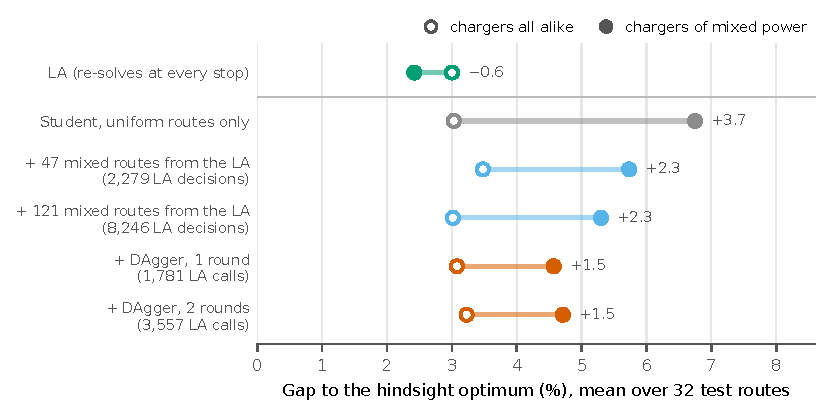
\includegraphics[width=\textwidth]{fig_effort.pdf}
\Description{Dot chart with six rows. Each row joins a hollow dot, the mean
gap to the hindsight optimum on 32 test routes whose stations have the same
power, to a filled dot, the same routes with stations of different powers.
Look-ahead: 3.0 to 2.4 percent. Network trained on uniform routes only: 3.0 to
6.8. With 47 routes from the look-ahead: 3.5 to 5.7. With 121: 3.0 to 5.3.
With one round of data aggregation: 3.1 to 4.6. With two rounds: 3.2 to 4.7.}
\caption{Mean gap to the oracle of the network on the 32 test routes, with
stations of equal power (hollow) and of different powers (filled), depending on
the additional training data. The number is the increase in percentage
points. Paired statistics are given in Table~\ref{tab:mixed}.}
\label{fig:effort}
\end{figure}

\subsubsection{Results.}
Table~\ref{tab:mixed} shows that the LA does not suffer from the variation in
power: its gap decreases slightly, because it takes 81\% of its energy at
700 and 1000\,kW stations and only 3\% at 150\,kW stations. In contrast, all
policies trained on routes with equal powers lose at least 3.7 percentage
points, and the trees distribute their charging almost evenly over the
stations. On a route with equal powers, the features of the current station
and of the next ones always coincide, so that the data contain no information
on how to choose between stations of different powers. Neither the 49
additional features nor a network architecture that evaluates every station
with a shared sub-network and compares the current station with the best
reachable one closed this gap; the latter showed an advantage on the
validation routes that did not hold on the test routes.

\subsubsection{Additional demonstrations versus data aggregation.}
We then compared two ways of using the LA on routes with varying powers
(Table~\ref{tab:mixed} and Fig.~\ref{fig:effort}): adding the LA's runs on 47
or 121 such training routes, or applying Algorithm~\ref{alg:dagger} on the
47 short training routes. Additional demonstrations reduce the increase from
3.7 to 2.3 percentage points, but 3.6 times more LA decisions bring no further
improvement. One round of data aggregation, with 1{,}781 LA queries, reduces
the increase to 1.5 percentage points. It is the only configuration whose
improvement over the network trained on uniform routes is clearly larger than
the noise ($2.2\pm0.7$ points), and it is at least as good as additional
demonstrations ($0.8\pm0.9$ points better than with 47 routes, $0.8\pm1.2$
better than with 121). A second round reduces the variance across training
seeds but not the mean. The labels collected in this way are specific to the
policy that visited the states: the same labels do not improve the trees
($+5.2\pm1.4$, against $+3.6\pm1.3$ with 121 additional routes). On routes
where both the power and the distance between stations vary, the benefit of
data aggregation is smaller, since it was only applied to routes with varying
power. None of these additions degrades the base case: all models remain
within noise of the LA on the 125 base-case test routes, without violation.

\subsubsection{Remaining gap.}
After either kind of additional data, the learned policy remains about two
percentage points behind the LA on these routes (Table~\ref{tab:mixed}, last
column). Note that on the first eight routes solved by the LA, the learned
policy appeared to be within one point of it; the larger sample does not
confirm this. The variability of the LA itself, whose route durations differ
by 0.35\% (median) between two runs on the same route and realization, is of
the same order as several of the effects reported here.

\section{Conclusion}
\label{sec:conclusion}

In this work, we studied a policy learned by imitation of a stochastic
look-ahead for the joint scheduling of charging, breaks and daily rests of an
electric truck. Using the costs computed by the look-ahead for every
candidate action, and enforcing the regulation through a symbolic shield, the
learned policy matches the look-ahead on held-out routes, never violates the
regulation, and decides in a few milliseconds. It generalizes to battery
capacities, charger powers and station spacings within the training range,
but not to slower chargers or to routes on which charger power varies. In the
latter case, data aggregation with the look-ahead as expert is the most
efficient use of solver time among the options we tested, and recovers about
half of the loss. The remaining gap of about two percentage points did not
decrease with more data of either kind. A natural extension is a hybrid
policy that calls the look-ahead only for the charging decisions on such
routes. The main limitations of this study are the synthetic instances, the
size of the sample of routes with varying powers (32), and the use of a single
training seed for the trees in Sects.~\ref{sec:physics} and~\ref{sec:mixed}.

\begin{credits}
\subsubsection{\ackname}
% TODO: funding
\subsubsection{\discintname}
The authors have no competing interests to declare that are relevant to the
content of this article.
\end{credits}
%
\bibliographystyle{splncs04}
\bibliography{references}
\end{document}
